% taux_cases.tex — the four canonical depth-profiles of the shear-stress gradient τ_zx,x(ζ)
% in a partially yielded bending plate (Eq. taux_two of the manuscript):
%   τ_zx,x = (3V'/4c³)(c²−ζ²)  [load term]  +  (3Vc'/4c⁴)(3ζ²−c²)  [core-narrowing term]
% Panels: (a) c'=0 load only; (b) V'=0 narrowing only; (c) reinforcing signs; (d) opposing signs.
% All profiles are even in ζ: centre of mass stays at the midplane (dot). c = 0.6·(h/2).
% Compile: tectonic taux_cases.tex
\documentclass[border=8pt]{standalone}
\usepackage{amsmath}
\usepackage{tikz}
\usetikzlibrary{arrows.meta}
\begin{document}
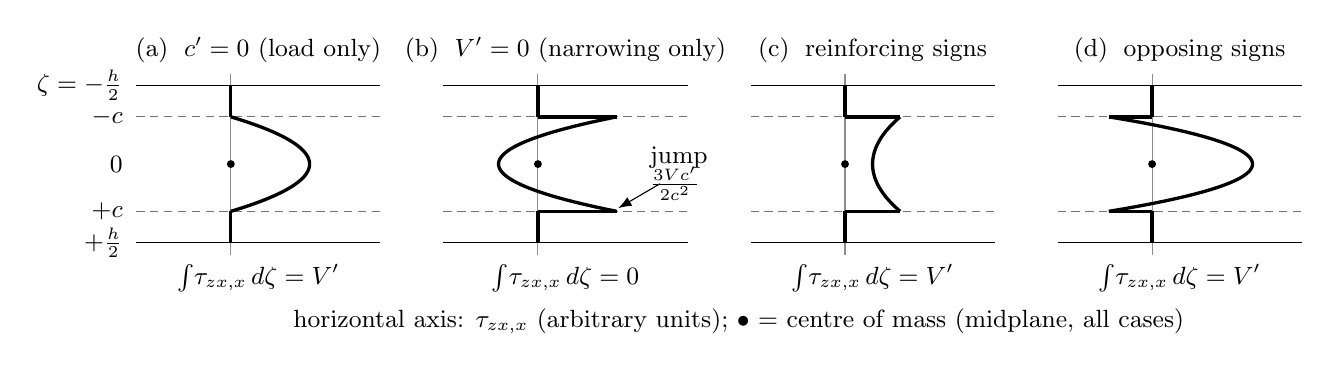
\begin{tikzpicture}[>=Latex,scale=1.0]
  \def\c{0.6}     % elastic core half-width (units of h/2 = 1)
  \def\W{2.1}     % panel horizontal half-range for the profile amplitude
  \def\gap{3.9}   % panel spacing

  % T_a(ζ) = (c²−ζ²)/c²  (load, max 1 at centre, 0 at ±c)
  % T_b(ζ) = (3ζ²−c²)/(2c²) (narrowing, −1/2 at centre, +1 at ±c, zero integral)

  \foreach \p/\Aa/\Bb/\ttl/\res/\jmp in {%
      0/1.0/0.0/{(a)\; $c'=0$ (load only)}/{$\int\!\tau_{zx,x}\,d\zeta = V'$}/0,
      1/0.0/1.0/{(b)\; $V'=0$ (narrowing only)}/{$\int\!\tau_{zx,x}\,d\zeta = 0$}/1,
      2/0.7/0.7/{(c)\; reinforcing signs}/{$\int\!\tau_{zx,x}\,d\zeta = V'$}/1,
      3/1.0/-0.55/{(d)\; opposing signs}/{$\int\!\tau_{zx,x}\,d\zeta = V'$}/1}{
    \begin{scope}[shift={({\p*\gap},0)}]
      % plate band and core
      \draw[thin] (-1.2,1) -- (1.9,1);      \draw[thin] (-1.2,-1) -- (1.9,-1);
      \draw[densely dashed,black!55,thin] (-1.2,\c) -- (1.9,\c);
      \draw[densely dashed,black!55,thin] (-1.2,-\c) -- (1.9,-\c);
      % zero axis (vertical)
      \draw[thin,black!45] (0,-1.15) -- (0,1.15);
      % profile: exterior (zero) segments — idealized truncation
      \draw[very thick] (0,\c) -- (0,1);
      \draw[very thick] (0,-\c) -- (0,-1);
      % profile inside the core: x = A·T_a(ζ) + B·T_b(ζ), plotted horizontally
      \draw[very thick] plot[domain=-\c:\c,samples=80]
        ({\Aa*((\c*\c-\x*\x)/(\c*\c)) + \Bb*((3*\x*\x-\c*\c)/(2*\c*\c))},\x);
      % jump connectors at ζ = ±c (edge value = A·0 + B·1 = B)
      \ifnum\jmp=1
        \draw[very thick] ({\Bb},\c) -- (0,\c);
        \draw[very thick] ({\Bb},-\c) -- (0,-\c);
      \fi
      % centre-of-mass marker at the midplane
      \fill (0,0) circle (0.05);
      % labels
      \node[align=center] at (0.35,1.45) {\small \ttl};
      \node at (0.35,-1.45) {\small \res};
    \end{scope}
  }

  % shared vertical-axis labels (left of panel a)
  \node[left] at (-1.25,1)    {\small $\zeta=-\tfrac{h}{2}$};
  \node[left] at (-1.25,\c)   {\small $-c$};
  \node[left] at (-1.25,0)    {\small $0$};
  \node[left] at (-1.25,-\c)  {\small $+c$};
  \node[left] at (-1.25,-1)   {\small $+\tfrac{h}{2}$};
  % jump annotation on panel (b)
  \draw[->,thin] (1*\gap+1.55,-0.25) -- (1*\gap+1.02,{-\c+0.04});
  \node[align=left,right] at (1*\gap+1.3,-0.12) {\small jump\\[-2pt]\small $\tfrac{3Vc'}{2c^{2}}$};
  % horizontal axis note under panel row
  \node at (1.5*\gap+0.6,-2.0) {\small horizontal axis: $\tau_{zx,x}$ (arbitrary units); $\bullet$ = centre of mass (midplane, all cases)};
\end{tikzpicture}
\end{document}
